\documentclass[a4paper,10pt]{article}
\usepackage[utf8]{inputenc}


% For the \todo{} command.
\usepackage{todo}

% Nice fonts
\usepackage{palatino}
% For doubled lines in tables.
% Useful for separation of table header from table body.
\usepackage{hhline}
\usepackage[english]{babel}
\usepackage{tabularx}
% Needed for Listings package with Eiffel.
% \usepackage{xcolor}
% Source code listings.
\usepackage{listings}
% Appendix with extra title.
% \usepackage [page] {appendix}
% To include PNG files.
\usepackage{graphicx}
% Nice looking captions.
\usepackage[font={footnotesize,sl}, labelfont=bf] {caption}
% Include PDF pages.
% \usepackage{pdfpages}

% Clickable links. Has to be the last package:
\usepackage [hidelinks] {hyperref}


\lstset{language=C,basicstyle=\ttfamily\small}


\newcommand{\todoref}{\todo{ref}}
\newcommand{\filepath}[1]{\emph{ #1}}

% Title Page
\title{Advanced Operating Systems \\ Project Report}
\author{Roman Schmocker \\ Yauhen Klimiankou}


\begin{document}

\maketitle


\section{Introduction}

This report provides documentation for the operating system which we built as part of the project in the Advanced Operating Systems course.
The code is based on a stripped-down version of Barrelfish \cite {web:barrelfish}.

This document is intended to describe the most important concepts and data structures in our code.
The idea is to give a high-level overview over the individual modules and serve as a complement for the comments within the code.
We will not however provide a detailed description of the API of every function, as this can be either looked up in the header file or generated with Doxygen \cite{web:doxygen}.

Section \ref{sec:getting-started} describes the required steps to compile the project and access basic system services.
The remaining sections of the report describe the individual project milestones.

\section{Getting started}
\label{sec:getting-started}

To be able to boot the operating system you need at least the following modules:
\begin{itemize}
 \item Kernel: armv7/sbin/cpu\_omap44xx
 \item Init: armv7/sbin/init
 \item Serial driver: armv7/sbin/serial\_driver
 \item Shell: armv7/sbin/memeater
 \item Filesystem: armv7/sbin/mmchs
\end{itemize}

It might be possible to run the project without a filesystem, but some commands fail.
We also provide a set of optional applications:
\begin{itemize}
 \item Hello World application: armv7/sbin/hello\_world
 \item Memory test: armv7/sbin/memtest
 \item Server test: armv7/sbin/test\_domain
 \item File Read Benchmark: armv7/sbin/fsb
\end{itemize}

Once the operating system has successfully booted control is transferred to a shell.
A detailed list of available commands is described in Table \ref{tbl:icl}.
Besides the builtin commands it is also possible to start the above optional applications by just typing their name without any prefix.

To get a channel to a system service one has to call \lstinline!aos_find_service! and \lstinline!aos_rpc_init!.
The channels to init and the serial driver are always available and can be retrieved with predefined functions.

Listing \ref{listing:channel-setup} shows a very small program to set up RPC channels.

\begin{lstlisting}[language=C, caption={Setup code for channels.}, captionpos=b, label=listing:channel-setup]
#include <barrelfish/aos_rpc.h>

struct aos_rpc* init_channel;
struct aos_rpc* serial_channel;
struct aos_rpc filesystem_channel;

int main(int argc, char *argv[])
{
  // Get init and serial driver channel.
  init_channel = aos_rpc_get_init_channel ();
  serial_channel = aos_rpc_get_serial_driver_channel ();
  
  // Get the filesystem channel.
  // NOTE: Error handling omitted.
  struct capref fs_cap;
  aos_find_service (aos_service_filesystem, &fs_cap);
  aos_rpc_init (&filesystem_channel, fs_cap);
}
\end{lstlisting}

\section{Paging}

% 
% - Intent: quick lookup of page table, ``unmap'' requests from memory server
% 
% - Data structues
% -- Simple for virtual memory
% -- 2-level array for page tables (mirroring actual page tables)
% -- linked list for frames
% 
% - Problem: No unmap from domain itself
% -- esp. no recycling of virtual addresses
% -- we thought that malloc would never return memory anyway
% -- didn't think about domain spawning / bulk transfer with explicit map/unmap operations

The paging code is mostly contained in \filepath{lib/barrelfish/paging.c} and the corresponding header file.
The central element is the \lstinline!paging_state! struct.
When designing the data structure for the paging code we wanted to support the following functions in constant time:

\begin{itemize}
 \item Check if an address is valid.
 \item Lookup of the page tables associated to the virtual address.
 \item Allocation of a physical frame for a page.
 \item Deallocation of a frame when the memory server asks for it.
\end{itemize}

To support the first use case we just keep track of the allocated range of virtual addresses using two integer variables.
That way determining if a page fault is ``valid'' is very simple: 
If it's in the range, everything is ok and we can map the page to a frame, and if not we abort due to an invalid address.

The data structure of choice to represent the page table structure is a two-level array that mirrors the actual page tables.
Currently we only store the capability to the page tables and whether a certain page has been allocated at some point.
We don't yet store any flags, pointers to a swap file or other metadata, but it would be easy to add this information.

Frame management is a bit more complex, because we always do allocations of 1 MiB.
That way we can avoid an IPC call for every single page fault, but we also have to keep track of free and allocated space within a frame.
The \lstinline!struct frame_list! manages this information for a single frame.
To support the last use case it also keeps track of the actual pages stored on this frame.
The \lstinline!paging_state! struct then maintains a double ended queue of \lstinline!frame_list! nodes, where only the frame at the head of the list may contain some free space.

As already mentioned, an important use case we had in mind were requests to return a frame from the memory server.
We never implemented that functionality, but the data structure is designed to support it.
An implementation would have to do the following:
\begin{itemize}
 \item Remove the last \lstinline!frame_list! element.
 \item Write all pages backed by this frame to disk.
 \item (Optionally) update some flags and metadata in the page table array.
 \item Return the frame to the memory server.
\end{itemize}

The data structures used to track frames and page tables need some form of dynamic memory management.
Unfortunately however we can't use malloc/free in our paging implementation, because this memory is not initially mapped.
Therefore we used slab allocators (from \filepath{include/barrelfish/slab.h}) to manage the memory needed by these data structures.
The \lstinline!memory_refill! function in our paging code is used to enlarge the pool of usable memory if the slab allocators run out of space.

\subsection{Assessment}

Our initial design of the paging module turned out to be rather flexible.
Over the course of the project, we only had to change small things, like adding another slab allocator for exception stacks of user-level threads 
or implementing \lstinline!paging_map_fixed_attr!, where we could adapt an existing function that did almost the same job.

The only thing that proved to be insufficient was the management of virtual address space.
The initial assumption that only malloc/free can issue unmap operations (and never does as it's not implemented) was wrong.
There are some parts in the code that directly interacts with the paging library and needs to ``free'' a range of virtual memory sometimes, among them the spawndomain library or the bulk transfer mechanism.

Supporting this would have required us to rewrite a lot of existing code, and that's why we didn't do it in the end.
This in turn means that our current solution leaks virtual addresses, but we tried to reduce this as much as possible by reusing the ranges of virtual memory.

\section{Local Message Passing}

The local message passing (LMP) system is mostly implemented in \filepath{lib/barrelfish/aos\_rpc.c} for the client side.
Some generic server-side features are implemented in \filepath{lib/aos\_support/server.c}.

The LMP system has some important characteristics:
\begin{itemize}
 \item All messages are synchronous, i.e. receive is blocking.
 \item The channels are always one-to-one connections.
 \item The communication is client-server style.
 \item We support direct connections to any server (i.e. no indirection through init).
 \item Every ``send'' message has an enum constant as its first argument that denotes the message type.
 \item Every ``reply'' message has an error code as its first argument.
 \item All other arguments are determined by the actual message type.
\end{itemize}

The individual message types and their arguments are described in the header file \filepath{include/barrelfish/aos\_rpc.h}.
To support writing code on the client side we implemented the feature \lstinline!aos_send_receive! which takes a struct containing all arguments, 
sends a request to the server, waits for a reply, and copies the receive arguments back into the struct.
That way we could avoid some code duplication for every remote procedure call.

Some servers provide core system services which need to be available in every program.
Init for example provides RAM, and the serial driver provides I/O.
We therefore set up some predefined channels to these services which are initialized in \filepath{lib/barrelfish/init.c}.
The channels can be accessed with functions defined in \filepath{aos\_rpc.h} (see Section \ref{sec:getting-started}).
% The channels can be retrieved with the functions \lstinline!aos_rpc_get_init_channel! and \lstinline!aos_rpc_get_serial_driver_channel!, respectively.

\subsection{Connection setup and name service}

In our LMP implementation we wanted to support direct channels between two domains.
To do that we had to implement some additional functionality, in particular a simple name service and a mechanism to set up a new connection.

The design of the name service is very simple.
In \filepath{aos\_rpc.h} we added an enum type \lstinline!aos_service! which is used for some of the core system services, such as the serial driver or the FAT file system.
Each domain that acts as a server for such a core system service then has to register itself via the \lstinline!AOS_RPC_REGISTER_SERVICE! LMP message.
Init itself keeps track of all registered servers and therefore acts as a name service.

When a client wants to find a particular service, it sends a request to init, and init replies with a new endpoint capability of the specified domain.
This was a bit tricky to implement, because we only allow one-to-one connections, so init first has to request a new endpoint from the (registered) server.
Init shouldn't mix the reply however with some other request from another domain, therefore we had to break our usual send-reply protocol and plan this interaction carefully.

In a step-by-step fashion this is what happens when a domain wants to find, for example, the serial driver:

\begin{itemize}
 \item The client sends an \lstinline!AOS_RPC_FIND_SERVICE! with the enum constant of the serial driver to init.
 \item Init uses a new request ID (a ``cookie'') and remembers the channel that sent the request.
 \item Init checks if the serial driver is registered. 
 If this is the case it sends an \lstinline!AOS_ROUTE_REQUEST_EP! to it, which includes the previously generated request ID.
 \item The serial driver handles the enpoint request call by creating a new channel.
 It replies to init with an \lstinline!AOS_ROUTE_DELIVER_EP! containing the new endpoint and the unchanged request ID as arguments.
 Note that this RPC call doesn't follow the usual send-reply style message exchange, because the reply contains a message type argument.
 \item Thanks to the special reply format init can handle the request like any other LMP message.
 When receiving the \lstinline!AOS_ROUTE_DELIVER_EP!, init retrieves the channel that initially sent the \lstinline!AOS_RPC_FIND_SERVICE! request using the request ID and forwards the endpoint.
 \item The client domain wakes up again receives the new endpoint, which it can then use to establish a direct connection.
\end{itemize}


% - Synchronous message passing, one-to-one
% - channels between any client/server possible (not just init)
% - general format: service identifier, args -> reply: error code, args
% - aos\_rpc.c: client API
% -- support feature \lstinline!aos_send_receive!
% -- only initialize arguments and receive result.
% - aos\_support/server.c: generic server support routines
% - routing: in init - service registration, find requests
% - bulk transfer: shared buffer, bound to a channel
% - predefined channels (provided by libbarrelfish): init, serial\_driver


\subsection{Bulk transfer}

For a long time throughout the project we only had the basic message-passing communication model.
Although this worked well, we always had to split an IPC call into several messages if the data to be transmitted exceeded the capacity of a single message.
This was a tedious and error prone process, and due to this we decided to add a mechanism for bulk transfer.

The basic idea is to set up a buffer which is shared between client and server.
This setup is initiated by the client, and only when it is actually needed.

We added a new message type which allowed a client to share a frame with a buffer and get back a \lstinline!memory_descriptor!, which it can use afterwards for other IPC calls.
The server-side part is implemented in \filepath{lib/aos\_support/}, which had the nice side effect that every server gained the buffer sharing mechanism for free without any further changes.
The client-side part is implemented in \filepath{lib/barrelfish/aos\_rpc.c}, where it is now possible to ``attach'' a shared buffer to any \lstinline!struct aos_rpc! channel.

The bulk transfer mechanism was a pretty late addition to the code base, therefore not all RPC calls have been changed to make use of it yet.

\section{Shell}
The shell is the standard tool for communication and interaction between user and operating system.
It is the only user interface currently existing in our OS.
  
Historically the shell was part of the memeater module, which was used to test the paging code.
It completely lost its original functionality at some point however, and the only thing remaining is the name.
The source code can be found at \filepath{usr/memeater/memeater.c}.

The main difference in our shell compared to a usual Linux shell is that it uses the serial port interface (also knows as RS-232) for input and output.
%it is remote shell which uses the host system as an source of input and target for output streams. 
% Communication with the host computer system goes through serial port interface (also knows as RS-232) for which incoming stream of characters is treated as a standard input stream and outgoing set of characters is treated as a standard output stream in terms of C language. 
% Host computer system is such design plays o role of conventional terminal by connecting the input stream stream of characters from the serial port with display and pushing the characters inputted from keyboard to the same serial port.
The Picocom \cite{web:picocom}
 utility is used at the other end of the serial connection to display and send characters.

Communication through the serial port is implemented in an independent server, located at \filepath{usr/serial\_driver/}.
The shell interacts with this driver using the RPC calls \lstinline!aos_rpc_serial_getchar! and \lstinline!aos_rpc_serial_putchar! and some support functions from the standard C library.

Like in most servers the exection of the shell consists of three phases:
\begin{enumerate}
	\item Initialization.
	\item Service loop.
	\item Deinitialization.
\end{enumerate}

During the initialization phase the shell sets up its global state and establishes connections to other system components which will be used in its main loop.
The shell uses the following system services:
\begin{enumerate}
	\item Filesystem
	\item LED Driver
	\item Process Manager
	\item Serial Driver
\end{enumerate}
% Global variables within the shell are:
% \begin{enumerate}
% 	\item A boolean sign for termination.
% 	\item A string describing the current directory.
% \end{enumerate}

The service loop of the shell is an endless loop which can only be exited when the global flag \lstinline!shell_running! is set to \lstinline!false!
Each iteration of the loop handles one input request and consist of several steps:
\begin{enumerate}
	\item Assembling the request string.
	\item Splitting the request into two parts: command and arguments.
	\item Lookup of the handler function.
	\item Execution of the request.
\end{enumerate} 

The purpose of the first step is to split the endless input stream from the serial port into separate strings, where each one represent single request.
The ASCII carriage return character is used as a separator between sequential requests.
This split is implemented in function \lstinline!receive_request!, which also echoes every incoming character back to the serial port.
The echo functionality enables users to see what they type.
% and by this control correctness of input and reply for the inputted request from the shell running on Pandaboard.

Unfortunately we don't support special treatment of some control characters (like backspace) yet.
As a result a typo in the input can only be fixed by flushing the current wrong request and retyping it again.
Once the full request is assembled it is passed to the next step of within the service loop.
  
To facilitate request processing we split it into a command and an arguments part.
The command part is considered as the first word of a request, whereas arguments is the remainder.
Any space characters between command and arguments are omitted.
Currently the shell doesn't split the argument string any further.
It is the responsibility of each command handler to split and process arguments in an appropriate way. 

The shell distinguishes between internal and external commands.
Internal commands are embedded and executed by the shell itself.
A list of internal commands can be found in table \ref{tbl:icl}.
The lookup of an internal command is implemented as a simple loop through the internal command list until an entry with the same name is found. 

\begin{table}[h]
	\centering
	\begin{tabular}{| m{2.0cm} | m{1.5cm} | m{7.0cm} |}
		\hhline{===}
		\textbf{Command} 	& \textbf{Args} 	& \textbf{Description}	\\
		\hhline{===}
		cat 				& file path 							& Display the content of the specified file.\\ \hline
		cd 				& ---  & Set the current directory to / \\ \hline
		cd 				& file path &  Set the current directory to the absolute or relative path specified by the argument.	\\ \hline
		echo 				& string 							& Display the argument string. \\ \hline
		exit 				& --- 							& Exit the shell. \\ \hline
		kill 				& integer 							& Force termination of the process with the PID specified as an argument. Init (PID 0) can't be terminated. \\ \hline
		ledoff			& ---								& Turn off the LED on the Pandaboard.\\ \hline
		ledon				& --- 							& Turn on the LED on the Pandaboard.\\ \hline
		ls 				& --- 							& Display list of files and directories in the current directory. \\ \hline
		oncore			& integer, string 					& Execute the specified external command on the kernel which the given ID. Can be used to execute programs on the second kernel.\\ \hline
		ping 				& --- 							& Send a series of `ping' messages to the `test\_domain' process. Expects the latter to be running.\\ \hline
		ps 				& --- 							& Display the currently running processes.\\ \hline
		run\_memtest		& integer 							& Run a memory allocation test. Allocates and fills a memory chunk of the specified size.\\ \hline
		test\_string		& --- 							& Send a long predefined string to the serial driver display it.\\ \hline            		
	\end{tabular}
	\caption{List of shell internal commands}
	\label{tbl:icl}
\end{table}


A command that does not match against an internal command is treated as an external command.
When encountering an external command the shell tries to find and spawn a process with the same name in the boot image.

External commands can be executed in two modes: background and foreground.
By default the shell execute commands in foreground mode, but background mode can be enabled by putting the `\&' character at the end of the request.
When a command runs in foreground mode the shell suspends itself until the spawned domain terminates.
The right to receive characters on the serial port is also transferred to the foreground domain.
A command running in background runs concurrently with the shell and does not get access to the input system.
    	    	
\section{Serial I/O}
The serial driver is a mediator between serial port connection and the rest of the operating system.
t is located in \filepath{usr/serial\_driver/}.
It has a straightforward implementation due to the simplicity of the serial port management, at least on our level of use.
The driver doesn't support buffering, interrupts, baud rate control etc. and relies to the preliminary initialization made by the kernel at boot time.
The driver uses polling to receive characters on the serial port.

The driver serves as a target for the following RPC calls and services:
\begin{enumerate}
	\item Send a character over serial port.
	\item Receive a character from the serial port.
	\item Send a string over the serial port. This makes use of the bulk transfer mechanism to avoid splitting and transmitting the string in small chunks.
	\item Set a domain as foreground domain. The specified domain will then be the only one with the right to receive input from the serial port.
\end{enumerate}

In addition libc was adapted to use the serial port driver as a backend for \lstinline!printf!, \lstinline!scanf! and related functions.
As a result any application is able to use traditional C-like IO with our serial driver.

\section{Process management}
\label{sec:process-management}

Spawning and managing domains is done in init.
The code can be found in \filepath{usr/init/process\_manager.c}, \filepath{usr/init/main.c} and \filepath{lib/aos\_support/module\_manager.c}.
The latter keeps track of the modules shipped with the multiboot image and maps them into init's address space.

The process manager is responsible to spawn a new domain and keep track of all running domains.
The main data structure within the process manager is the \lstinline!domain_info! struct.
It keeps track of a domain's state, its dispatcher and CSpace, and its channel to \emph{init}.

The most important function is \lstinline!spawn!, which takes the name of a domain as an argument.
The function does all the steps required to spawn a new domain:
\begin{itemize}
 \item Loading the multiboot module.
 \item Setting up the Dispatcher, CSpace and VSpace.
 \item Parse and relocate the ELF image.
 \item Create the channel between init and the new domain.
 \item Store all relevant data in the \lstinline!domain_info! struct.
 \item Make the domain runnable.
\end{itemize}

The process manager maintains an array of \lstinline!domain_info! structs to keep track of all spawned domains.
The array index serves as a unique domain identifier.
If the initial length of the array is insufficient it can be dynamically grown, which means we don't have a hard limit on the number of possible domains.
The \lstinline!ps! command dumps the name and domain ID of every domain stored within the array.

\subsection {Domain Teardown}

Tearing down a domain is challenging in Barrelfish.
The first issue we had to solve is to realize \emph{when} a domain needs to be cleaned up, i.e. we needed to get some notification that a domain has stopped running.
To solve this problem we added a new IPC call \lstinline!AOS_RPC_KILL! which can be used to kill a domain, given a domain ID.
We then adapted \lstinline!libc_exit! in \filepath{lib/barrelfish/init.c} to perform this call with its own ID (or in other words: the domain commits suicide).

Init therefore gets a notification that some domain wants to be killed.
It can then revoke the dispatcher capability to make the domain unrunnable.

The next step would be to properly clean up the domain.
This would consist of returning all frames and device frames to the corresponding server and revoke the root CNode to clean up the capability space.
We could only implement the last part however, as keeping track of allocated frames for each domain would have required us to do some major refactoring.
This in turn means that we're leaking memory for each spawned domain, and it's the reason why a domain never leaves the \emph{zombie} state as for now.

The introduction of \lstinline!AOS_RPC_KILL! allowed us to introduce another mechanism.
A domain can now issue an \lstinline!AOS_RPC_WAIT_FOR_TERMINATION! to get a notification as soon as another domain stops.
The shell makes use of this facility to suspend itself during foreground tasks.
And because we already had the \lstinline!AOS_RPC_KILL! call we could also very easily extend our shell to spawn process in the background and \emph{kill} them later.

\subsection{Assessment}
Our domain management code went through many refactorings, and we're still not quite happy.
The main problem is to properly clean up a zombie domain.

It would be necessary to keep track of frames and device frames allocated by that domain and return them to the servers upon teardown.
This would have meant to introduce a lot more state and changes in existing IPC calls to keep track of allocated frames.
A potential problem is the bulk transfer mechanism, where frames are shared between client and server, and it might not be that easy to revoke these frames.
With some more time we may have been able to find a solution, but it's certainly not an easy task.

% - currently done in init
% - server manages process table and info about loaded modules
% -- can be printed with ps command
% - shell attempts to start program with specific name if command not recognized
% - mechanism to register for end notification (foreground tasks)
% - kill command to revoke dispatcher capability (background tasks)
% - no further cleanup for zombie domains as for now

\section{Mupltiple Cores}

\subsection{Preparing the kernel image}

The preparation of the kernel image is mostly done in \filepath{usr/init/cross\_core\_setup.c}.
The implementation is heavily inspired\footnote{copy-pasted} from the upstream Barrelfish code base.
Compared to the upstream mechanism we implemented some simplifications however, since we don't have to support more than two cores.
We also adapted the code a bit to our own data structures.

\subsection{Low-level mechanisms}
\label{sec:low-level-mechanisms}

To start the second core one has to call the \lstinline!sys_boot_core! system call, which eventually executes \lstinline!start_aps_arm_start! in the first kernel.
Within this function there's no magic going on - it just writes the start address for the second core to a register and issues an interrupt.

The real magic happens in \lstinline!arch_init! in \filepath{kernel/arch/omap44xx/init.c} and  \lstinline{arm_kernel_startup} in \filepath{kernel/arch/omap44xx/startup\_arch.c}.
In \lstinline!arch_init! we set up the \lstinline!global! struct which contains data to be shared between both kernels.
Among the data shared between the two kernels is the multiboot image.
We also reserve a region of physical memory as a buffer for future cross core communication and store the physical address and size of it in the \lstinline!global! struct.

In \lstinline!arm_kernel_startup! we do a static split of the available physical memory.
Each init thus only gets a capability to half of the memory, which prevents them from messing around with each others address space.
Finally, we also create the capability to the shared frame in this functions and store it in the \lstinline!TASKCN_SLOT_MON_URPC! slot.

\subsection{Inter-Kernel Communication}
	Inter-kernel communication (IKC) is a new type of communication subsystem introduced by the multikernel operating system design.
	Like inter-process communication links independent and isolated domains running in the same OS node, IKC links independent and isolated nodes in a multi-kernel operating system located on the same machine to a single system.
	These nodes are isolated due to the fact that all computer system resources (mainly CPU and memory) are logically split between kernels and each kernel manages and uses its own system resources. 
	Inter-kernel communication implements a communication channel using shared memory, because this is the fastest to communicate between CPUs on the same machine.
	
	In the context of the project a master-slave communication model was chosen for IKC. 
	The kernel running on Core 0,
	%(here and later we will use terms CPU and core interchangeably, because from the point of view of this project and from the point of view of software development in general multiprocessor system doesn't differ from the multicore-processor based system), 
	which is a bootstrap processor, plays role of the master whereas the kernel on Core 1 is the slave.
	
	When spawning the second kernel an IKC communication channel is established between kernels.
	We're using the reserved shared memory region described in Section \ref{sec:low-level-mechanisms} for that purpose.
	Communication over this channel is handled by communication drivers which control the data exchange.
	
	On both sides \emph{init} plays the role of IKC driver, but the behavior of master and slave differs.
	Communication can be initiated only by \emph{init} on the master kernel, where the main thread sends messages over channel and waits for a reply like a usual RPC call.
	
	On the slave side communication is handled by a special listener thread within \emph{init} which polls for new messages in the channel.
	The behaviour is similar to the server side of an RPC call: 
	It receives a message, handles it, sends a reply, and goes back to polling. 
	Currently the IKC server thread of the slave \emph{init} domain handles only one type of request: spawning new domains.
	
	The IKC channel is implemented as a full-duplex strictly-ordered channel for fixed size messages and FIFO service discipline. 
	The channel consist of two unidirectional subchannels with size 2Kb, one of which is used for messages from master to slave and the other one for messages in the opposite direction (look at Figure \ref{fig:ikc}).
	Both subchannels can be used concurrently at the same time.
	
	\begin{figure}[ht]
		\centering
   		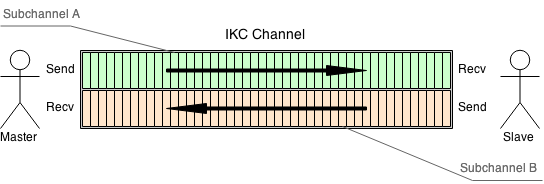
\includegraphics[width=\textwidth]{IKC_Structure.png}
		\caption{Inter-Kernel Communication Channel Design}
    		\label{fig:ikc}
	\end{figure} 
		
	There are three operations supported by channel:
	\begin{enumerate}
		\item Push: Put a message into the first free space in the send subchannel. 
		\item Pop: Receive and remove a message from the receive subchannel.
		\item Peek: Receive, but don't remove, a message from the receive subchannel.
	\end{enumerate}
	
	We chose to use a message size of 64 bytes. 
	We used this size for the following reasons:
	\begin{enumerate}
		\item It is aligned to the cache line size, where each message covers exactly two cache lines. 
		This property helps us to eliminate unwanted cache line flip-flopping which would reduce efficiency of communication.
		\item It is a power of two, which means that each subchannel contains exactly 32 message slots, which is also power of two. 
		This property allows us to easily and efficiently represent channels internally as a ring buffer.
		No single message can cross the boundary of the buffer, because the channel size is divisible by the message size and the message size is fixed.
		We can use integer overflow safely for read and write pointer tracking, because overflow will only occur in places of going back to the first slot of buffer. %TODO: Are you sure about that??
		All multiplication, division and modulo operations should be optimized by compiler by bit shifting and masking, which will replace expensive (especially on ARM) arithmetical operations by simple and cheap equivalents.
% 		If be honest we even not sure that ARM CPU used by Pandaboard provides hardware instructions for these operations or it relies on compiler which will implement them in software.
% 		In the same time we haven't checked that the expected behavior will be produced by compiler, because we haven't our binaries disassembled for explicit check (due to the lack of knowledge's of ARM assembler and appropriate disassembling software), but we sure that expected optimizations will be done, because it simple and well-known and this is exactly what we saw before for Microsoft Visual C++ compiler and IA-32 platform. 
		\item The message size allows to fit one LMP message into one IKC message.
		\item The second cache line is not often used for data transfer, so we reserve the last word for a ready sign.
		This allows us to reduce cache line flip-flopping between writer and reader, because the writer can fill the first cache line of the message without any distortion while the reader constantly checks the last word of second cache line. 
		When the writer has written whole message into channel, it will raise the ready flag at the end of the second cache line, notifying reader that it can read the message safely now.
% 		TODO: No - what if message size is bigger than one cache line (32 bytes)?
% 		As a result only three cache line passes between cores will occur: 2 line from reader to writer, 2 line from writer to reader and finally 1 line from writer to reader.
	\end{enumerate}
	
	Each endpoint of the channel uses a pair of channel pointers for receive and send. 
	The receive pointer is used for receive subchannel, and vice versa.
	Note that, for the same subchannel, the receive and send pointers are located on different cores and tracked independendly.
	

% - Spawning cores on low level.
% - Setup of ELF image
% - Communication between cores

\section{FAT file system}

The FAT filesystem is implemented in \filepath{aos\_support/fat32.c}, whereas the server and disk driver is located in \filepath{usr/mmchs/}.
We only support read operations on a FAT filesystem, and we didn't try to improve the block driver as well.

The main data structure for the FAT filesystem is the config struct:

\begin{lstlisting}
struct fat32_config {
    sector_read_function_t read_function;

    uint32_t volume_id_sector;
    uint32_t sectors_per_cluster;
    uint32_t fat_sector_begin;
    uint32_t cluster_sector_begin;
    uint32_t root_directory_cluster;
};
\end{lstlisting}

Within the struct we store some of the most important data, such as the start address of the File Allocation Table or the cluster region.
We also store a pointer to a function needed to read a block from disk.
That way we can easily reuse the FAT driver module for block devices other than the SD card of the Pandaboard.

A common operation in the FAT filesystem is to follow a chain of clusters and read consecutive sectors.
We introduced the \lstinline!struct sector_stream! to hide this complexity.
A sector stream is an iterator over a file or directory and can be advanced with \lstinline!stream_next!.

An important internal function is \lstinline!find_node!.
This function takes a path as an argument and tries to find a filesystem node (file or directory) with the given path.
If found it returns the start cluster and the file size (if it is a file) of the node.

\subsection{File management}
File operations are done in the usual open-read-close cycle and identified by a file descriptor.
When opening a file we call \lstinline!find_node! to search the filesystem for the file with the given path.
We then store a mapping from the file descriptor to the start cluster, the file size and the \lstinline!fat32_config!.

For file reads we use the \lstinline!sector_stream!.
We skip the first few sectors until we reach the position in the file requested by the user.
After that we just do a linear scan of the file and copy all bytes into a buffer.
To send the byte buffer back to the client we make use of the bulk transfer mechanism.

When closing a file we just discard the information collected during the open phase.

\subsection{Partition tables}
Due to the fact that Windows couldn't create an SD card without a partition table we had to add some rudimentary support for it.
The filesystem server loads the partition table and looks at the first partition table entry.
It then extracts the start block of the first partition and initializes the FAT driver with that information.

\subsection{ ELF loading}

Currently we don't support ELF loading.
The functionality is almost implemented, but we could not finish it in time.
The missing piece is a communication channel from init to the filesystem server, which is needed to get the binary of a channel.

Reusing the normal channel between init and the filesystem server is not possible without some refactoring, because init acts as a server in this channel.
Using the normal \lstinline!aos_rpc_find_servie! infrastructure isn't possible either, because init doesn't have a channel to itself.
The solution would have been to do some hack and create a new channel with init as a client and the filesystem as a server.

\todo {Write assessment}
\todo {Implement ELF loading}

% - filesystem code in aos\_support/fat32.c
% - handler in mmchs/filesystem\_server.c
% - Currently read-only
% - some support for partition tables
% - Performance improvements: sequential read? cached FAT? bulk transfer?

\section{Conclusion}
Throughout the project we've implemented central parts of an operating system.
We first implemented a module to do paging.
The next step was to implement an IPC mechanism which allowed us to do some simple message passing between processes.

We continued by implementing a shell and a user-space serial driver.
With the shell in place we added a mechanism to spawn and manage new processes.

We then added the functionality to boot the second core on the Pandaboard and implemented a communication channel between the two \emph{init} domains on each core.

Finally, we also added support to read a FAT file system on an SD card.

\begin{flushleft}
{{{
\bibliographystyle {plain}
\bibliography {./references}
}}}
\end{flushleft}


\todos

\end{document}          
 
